% One move by Mr X, from final_report.tex (fig:sequence), recoloured for the slides.
\documentclass[border=4pt]{standalone}
% Shared look for the slide diagrams: the deck's dark colours, sans text, transparent background.
\usepackage[scaled]{helvet}
\renewcommand{\familydefault}{\sfdefault}
\usepackage{tikz}
\usetikzlibrary{arrows.meta,positioning,fit,calc}
\definecolor{fg}{HTML}{F3F1EA}
\definecolor{muted}{HTML}{C9D2DC}
\definecolor{card}{HTML}{1A2430}
\definecolor{fin}{HTML}{243142}
\definecolor{edge}{HTML}{8C98A5}
\definecolor{amber}{HTML}{F5A524}
\definecolor{bg}{HTML}{111821}
\color{fg}

\begin{document}
\color{fg}
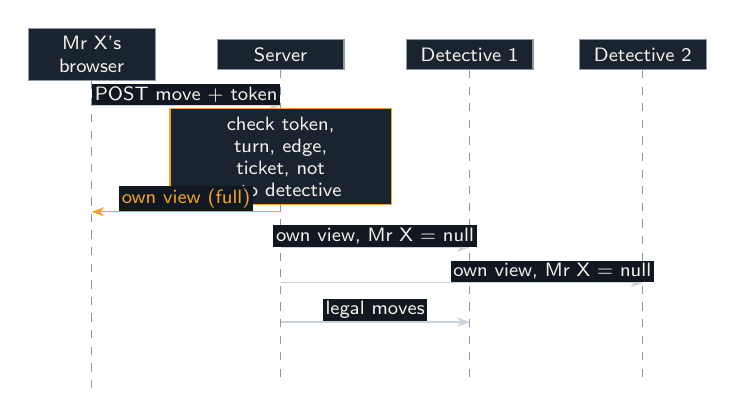
\begin{tikzpicture}[font=\scriptsize, arr/.style={-{Stealth[length=1.6mm]}, draw=muted},
  life/.style={draw=edge, dashed}, every node/.append style={fill=bg, inner sep=1pt, text=fg}]
  \foreach \x/\n/\l in {0/a/Mr~X's browser, 2.4/s/Server, 4.8/b/Detective~1, 7.0/c/Detective~2}{
    \node[draw=edge, fill=card, align=center, text width=14mm, inner sep=3pt] (\n) at (\x,0) {\l};
    \draw[life] (\n.south) -- ++(0,-3.9);
  }
  \draw[arr] (0,-0.65) -- node[above]{POST move + token} (2.4,-0.65);
  \node[draw=amber, fill=card, align=center, text width=26mm, inner sep=3pt] at (2.4,-1.3) {check token, turn, edge,\\ticket, not onto detective};
  \draw[arr, draw=amber] (2.4,-2.0) -- node[above, text=amber]{own view (full)} (0,-2.0);
  \draw[arr] (2.4,-2.45) -- node[above]{own view, Mr~X = null} (4.8,-2.45);
  \draw[arr] (2.4,-2.9) -- node[above, pos=0.75]{own view, Mr~X = null} (7.0,-2.9);
  \draw[arr] (2.4,-3.4) -- node[above]{legal moves} (4.8,-3.4);
\end{tikzpicture}
\end{document}
